%%%%%%%%%%%%%%%%%%%%%%%%%%%%%%%%%%%%%%%%%%%%%%%%%%%%%%%%%%%%%%%%%%%%%%%%%%%
\subsection{\label{sec:Globus-intro}Working with Globus}
%%%%%%%%%%%%%%%%%%%%%%%%%%%%%%%%%%%%%%%%%%%%%%%%%%%%%%%%%%%%%%%%%%%%%%%%%%%

The Globus software provides a well-defined set of protocols
that allow authentication, data transfer, and remote job submission.

Authentication is a mechanism by which an identity is verified.
Given proper authentication, authorization to use a resource
is required.
Authorization is a policy that determines who is allowed to do what. 


%%%%%%%%%%%%%%%%%%%%%%%%%%%%%%%%%%%%%%%%%%%%%%%%%%%%%%%%%%%%%%%%%%%%%%%%%%%
\subsubsection{\label{sec:Globus-Protocols}Globus Protocols}
%%%%%%%%%%%%%%%%%%%%%%%%%%%%%%%%%%%%%%%%%%%%%%%%%%%%%%%%%%%%%%%%%%%%%%%%%%%
Condor uses the following Globus protocols.
These protocols allow Condor to utilize grid machines for
the execution of jobs.
\begin{description}
\item[GSI]
The Globus Toolkit's Grid Security Infrastructure (GSI) provides essential
\index{Condor-G!GSI}
building blocks for other Grid protocols and Condor-G.
This authentication and authorization system
makes it possible to authenticate a user just once,
using public key infrastructure (PKI) mechanisms to verify
a user-supplied grid credential.
GSI then handles the mapping of the grid credential to the
diverse local credentials and authentication/authorization mechanisms that
apply at each site. 
\item[GRAM]
The Grid Resource Allocation and Management (GRAM) protocol supports remote
\index{Condor-G!GRAM}
submission of a computational request (for example, to run program P)
to a remote computational resource,
and it supports subsequent monitoring and control of the resulting
computation. 
\item[GASS]
The Globus Toolkit's Global Access to Secondary Storage (GASS) service provides
\index{Condor-G!GASS}
mechanisms for transferring data to and from a remote HTTP, FTP, or GASS server. 
Condor-G uses GASS to transfer the executable, 
\File{stdin}, 
\File{stdout}, and 
\File{stderr}
between the machine where a job is submitted and the remote resource.
\item[RSL]
RSL is the language GRAM accepts to specify job information.
\end{description}

%%%%%%%%%%%%%%%%%%%%%%%%%%%%%%%%%%%%%%%%%%%%%%%%%%%%%%%%%%%%%%%%%%%%%%%%%%%
\subsubsection{\label{sec:Grid-Access}Accessing the Grid with Condor-G}
%%%%%%%%%%%%%%%%%%%%%%%%%%%%%%%%%%%%%%%%%%%%%%%%%%%%%%%%%%%%%%%%%%%%%%%%%%%

Condor-G allows the user to treat the Grid as a local resource,
and the same command-line tools perform basic job management such as:
\begin{itemize}
\item Submit a job, indicating an executable, input and output files,
and arguments
\item Query a job's status
\item Cancel a job
\item Be informed when events happen,
such as normal job termination or errors
\item Obtain access to detailed logs that provide a complete history of a job
\end{itemize}

These are features that Condor has provided for many years.
Condor-G extends this to the grid,
providing resource management 
while still providing fault tolerance and exactly-once execution 
semantics. 

\begin{figure}[hbt]
\centering
\includegraphics{grids/gfig1.eps}
\caption{\label{fig:condorg}Remote Execution by Condor-G on Globus managed resources}
\end{figure}

Figure~\ref{fig:condorg} shows how Condor-G interacts with Globus protocols.
Condor-G contains a GASS server, used to transfer the executable,
\File{stdin}, \File{stdout}, and \File{stderr} to and from
the remote job execution site.
Condor-G uses the GRAM protocol to contact the remote Globus Gatekeeper
and request that a new job manager be started.
GRAM is also used to monitor the job's progress.
Condor-G detects and intelligently handles cases
such as if the remote Globus resource crashes.

%%%%%%%%%%%%%%%%%%%%%%%%%%%%%%%%%%%%%%%%%%%%%%%%%%%%%%%%%%%%%%%%%%%%%%%%%%%
\subsection{\label{sec:Condor-G-Setup}Set Up of Condor-G}
%%%%%%%%%%%%%%%%%%%%%%%%%%%%%%%%%%%%%%%%%%%%%%%%%%%%%%%%%%%%%%%%%%%%%%%%%%%

%%%%%%%%%%%%%%%%%%%%%%%%%%%%%%%%%%%%%%%%%%%%%%%%%%%%%%%%%%%%%%%%%%%%%%%%%%%
\subsubsection{\label{sec:Condor-G-Install}Condor-G Installation}
%%%%%%%%%%%%%%%%%%%%%%%%%%%%%%%%%%%%%%%%%%%%%%%%%%%%%%%%%%%%%%%%%%%%%%%%%%%
\index{Condor-G!installation}
Condor-G is included in the standard Condor distribution.
Once Condor is obtained via download, installed, and configured,
(see
section~\ref{sec:install} on page~\pageref{sec:install})
there are two steps necessary before a globus universe job
can be submitted:

\begin{enumerate}

\item{Install Globus tools.}
Three ways are listed for obtaining the Globus tools:
   \begin{enumerate}
   \item{Globus}.
   From the web page at \URL{http://www.globus.org/}, follow links to the
   globus toolkit to get the resource management client bundle.
   \item{NMI}.
   From the web page at \URL{http://www.nsf-middleware.org/}, follow links
   to the NMI Release, and then to the Components, and finally to the
   Globus Toolkit. 
   \item{VDT}.
   From the web page at \URL{http://www.griphyn.org/vdt},
   follow the link to installing and setting up the Virtual Data Toolkit.
   \end{enumerate}

\item{Configure for Condor-G.}
If you installed Condor using the submit-only option, you will
need to add the following entries to your configuration file:
\begin{verbatim}
GRIDMANAGER             = $(SBIN)/condor_gridmanager
GAHP                    = $(SBIN)/gahp_server
MAX_GRIDMANAGER_LOG     = 64000
GRIDMANAGER_DEBUG       = D_COMMAND
GRIDMANAGER_LOG         = $(LOG)/GridLogs/GridmanagerLog.$(USERNAME)
GLIDEIN_SERVER_NAME     = gridftp.cs.wisc.edu
GLIDEIN_SERVER_DIR      = /p/condor/public/binaries/glidein
\end{verbatim}

If Condor-G is installed as root, the file
set by the configuration variable
\Macro{GRIDMANAGER\_LOG} must have world-write permission.
All of the parent directories for this file must
also have world-execute permission.
The Gridmanager runs as the user who submitted the job,
so the Gridmanager may not be able to write to the ordinary 
\MacroUNI{log} directory.
%The example configuration file sets the log file to be 
%\begin{verbatim}
%GRIDMANAGER_LOG = $(LOG)/GridLogs/GridmanagerLog.$(USERNAME) 
%\end{verbatim}
Use of the definition of \MacroNI{GRIDMANAGER\_LOG}
shown above will likely require the creation of
the directory \verb@$(LOG)/GridLogs@.
Permissions on this directory should be set
by running \Prog{chmod} using the value 1777. 

Another option is to locate the Gridmanager log files
somewhere else, like so:
\begin{verbatim}
GRIDMANAGER_LOG  = /tmp/GridmanagerLog.$(USERNAME)
\end{verbatim}

If you make any changes to the configuration file while
Condor is running, you will need to issue a \Condor{reconfigure}
command.

See section~\ref{sec:Configuring-Condor} on
page~\pageref{sec:Configuring-Condor} for
more information about configuration file entries.
See section~\ref{sec:Gridmanager-Config-File-Entries} on
page~\pageref{sec:Gridmanager-Config-File-Entries} for information
about  configuration file entries specific to the Condor-G
gridmanager.

\end{enumerate}

%%%%%%%%%%%%%%%%%%%%%%%%%%%%%%%%%%%%%%%%%%%%%%%%%%%%%%%
\subsubsection{\label{sec:Condor-G-Credentials}Credential Management}
%%%%%%%%%%%%%%%%%%%%%%%%%%%%%%%%%%%%%%%%%%%%%%%%%%%%%%%

%(Reword this section to talk more about credential management and less
%about specific config values. Also, probably move it out of the setup
%section.)

Condor-G periodically checks for an updated proxy at
an interval given by the configuration variable
\AdAttr{GRIDMANAGER\_CHECKPROXY\_INTERVAL}.
The value is defined in terms of seconds.
For example, if you create a 12-hour proxy, and then
6 hours later re-run \Prog{grid-proxy-init},
Condor-G will check the proxy within
this time interval, and use the new proxy it finds there.
The default interval is 10 minutes.

Condor-G also knows when the proxy of each job will expire,
and if the proxy is not refreshed before
\AdAttr{GRIDMANAGER\_MINIMUM\_PROXY\_TIME}
seconds before the proxy expires,
the Condor-G grid manager daemon exits.
Since the grid manager daemon keeps track of all jobs
associated with a proxy, its tasks
(such as authentication, file transfer, job log maintenance)
will not occur.
So, if
\AdAttr{GRIDMANAGER\_MINIMUM\_PROXY\_TIME}
is 180, and the proxy is 3 minutes away from
expiring, Condor-G will attempt to safely shut down,
instead of simply losing
contact with the remote job because Condor-G is unable to
authenticate the remote job.
The default setting is 3 minutes (180 seconds).

%%%%%%%%%%%%%%%%%%%%%%%%%%%%%%%%%%%%%%%%%%%%%%%%%%%%%%%%%%%%%%%%%%%%%%%%%%%
\subsection{\label{sec:Using-Condor-G}Using the Globus Universe}
%%%%%%%%%%%%%%%%%%%%%%%%%%%%%%%%%%%%%%%%%%%%%%%%%%%%%%%%%%%%%%%%%%%%%%%%%%%

\index{universe!Globus}
This section contains what users need to know to 
run and manage jobs under the globus universe.

%%%%%%%%%%%%%%%%%%%%%%%%%%%%%%%%%%%%%%%%%%%%%%%%%%%%%%%%%%%%%%%%%%%%%%%%%%%
\subsubsection{\label{sec:Running-CondorG-Job}Running a Globus Universe Job}
%%%%%%%%%%%%%%%%%%%%%%%%%%%%%%%%%%%%%%%%%%%%%%%%%%%%%%%%%%%%%%%%%%%%%%%%%%%
\index{Condor-G!job submission}

Under Condor, successful job submission to the Globus universe requires
credentials.
An X.509 certificate is used to create a proxy,
and an account, authorization, or allocation to use a grid resource
is required.
For more information on proxies and certificates,
please consult the Alliance PKI pages at 

\URL{http://archive.ncsa.uiuc.edu/SCD/Alliance/GridSecurity/}

Before submitting a job to Condor under the Globus universe,
make sure you have your Grid 
credentials and have used \Prog{grid-proxy-init} to create a proxy.

A job is submitted for execution to Condor using the
\Condor{submit} command.
\index{Condor commands!condor\_submit}
\Condor{submit} takes as an argument
the name of a file called a submit description file.
\index{submit description file!globus universe}
The following sample submit description file runs a job on
the Origin2000 at NCSA.

\begin{verbatim}
executable = test
globusscheduler = modi4.ncsa.uiuc.edu/jobmanager
universe = globus
output = test.out
log = test.log
queue
\end{verbatim} 

The 
\AdAttr{executable}
for this example is
transferred from the local machine to the remote machine.
By default, Condor transfers the executable, as well as any
files specified by the \AdAttr{input} command.
Note that this executable must be compiled for the correct
intended platform.

The \AdAttr{globusscheduler} command is dependent on the
scheduling software available on remote resource.
This required command will change based on the Grid resource
intended for execution of the job.
A jobmanager is the Globus service that is spawned at a remote site to
submit, keep track of, and manage Grid I/O for jobs running on the local
batch system there.
There is a specific jobmanager for each type of
batch system supported by Globus (examples are Condor, LSF, and PBS).

All Condor-G jobs (intended for execution on Globus-controlled
resources) are submitted to the globus universe.
The \verb@universe = globus@ command is required
in the submit description file.

No input file is specified for this example job.
Any output (file specified by the \AdAttr{output})
or error (file specified by the \AdAttr{error})
is transferred 
from the remote machine to the local machine as it is produced.
This implies that these files may be incomplete in the case
where the executable does not finish running on the remote resource.
The job log file is maintained on the local machine.

To submit this job to Condor-G for execution on the
remote machine, use
\begin{verbatim}
condor_submit test.submit
\end{verbatim}
where \File{test.submit} is the name of the submit description file.

Example output from 
\Condor{q} for this submission looks like:
\footnotesize
\begin{verbatim}
% condor_q


-- Submitter: wireless48.cs.wisc.edu : <128.105.48.148:33012> : wireless48.cs.wi

 ID      OWNER         SUBMITTED     RUN_TIME ST PRI SIZE CMD
   7.0   epaulson     3/26 14:08   0+00:00:00 I  0   0.0  test

1 jobs; 1 idle, 0 running, 0 held
\end{verbatim}
\normalsize

After a short time, Globus accepts the job.
Again running \Condor{q} will now result in

\footnotesize
\begin{verbatim}
% condor_q


-- Submitter: wireless48.cs.wisc.edu : <128.105.48.148:33012> : wireless48.cs.wi

 ID      OWNER         SUBMITTED     RUN_TIME ST PRI SIZE CMD
   7.0   epaulson     3/26 14:08   0+00:01:15 R  0   0.0  test

1 jobs; 0 idle, 1 running, 0 held
\end{verbatim}
\normalsize

Then, very shortly after that, the queue will be empty again,
because the job has finished:

\footnotesize
\begin{verbatim}
% condor_q


-- Submitter: wireless48.cs.wisc.edu : <128.105.48.148:33012> : wireless48.cs.wi

 ID      OWNER            SUBMITTED     RUN_TIME ST PRI SIZE CMD

0 jobs; 0 idle, 0 running, 0 held
\end{verbatim}
\normalsize


A second example of a submit description file runs the Unix \Prog{ls}
program on a different Globus resource.

\footnotesize
\begin{verbatim}
executable = /bin/ls
Transfer_Executable = false
globusscheduler = vulture.cs.wisc.edu/jobmanager
universe = globus
output = ls-test.out
log = ls-test.log
queue
\end{verbatim} 
\normalsize

In this example, the executable (the binary) has been pre-staged.
The executable is on the remote machine, and it is not to
be transferred before execution.
Note that the required 
\AdAttr{globusscheduler} and \AdAttr{universe}
commands are present.
The command
\begin{verbatim}
Transfer_Executable = FALSE
\end{verbatim}
within the submit description file identifies the executable
as being pre-staged.
In this case, the 
\AdAttr{executable}
command gives the path to the executable on the remote machine.

A third example submits a Perl script to be run as a submitted
Condor job.
The Perl script both lists and sets
environment variables for a job.
Save the following Perl script with the name \File{env-test.pl},
to be used as a Condor job executable.

\begin{verbatim}
#!/usr/bin/env perl

foreach $key (sort keys(%ENV))
{
   print "$key = $ENV{$key}\n"
}

exit 0;
\end{verbatim}

Run the Unix command
\begin{verbatim}
chmod 755 env-test.pl
\end{verbatim}
to make the Perl script executable.

Now create the following submit description file
(Replace \File{biron.cs.wisc.edu/jobmanager} with a resource
you are authorized to use.):

\footnotesize
\begin{verbatim}
executable = env-test.pl
globusscheduler = biron.cs.wisc.edu/jobmanager
universe = globus
environment = foo=bar; zot=qux
output = env-test.out
log = env-test.log
queue
\end{verbatim}
\normalsize

When the job has completed, the output file \File{env-test.out}
should contain something like this:

\footnotesize
\begin{verbatim}
GLOBUS_GRAM_JOB_CONTACT = https://biron.cs.wisc.edu:36213/30905/1020633947/
GLOBUS_GRAM_MYJOB_CONTACT = URLx-nexus://biron.cs.wisc.edu:36214
GLOBUS_LOCATION = /usr/local/globus
GLOBUS_REMOTE_IO_URL = /home/epaulson/.globus/.gass_cache/globus_gass_cache_1020633948
HOME = /home/epaulson
LANG = en_US
LOGNAME = epaulson
X509_USER_PROXY = /home/epaulson/.globus/.gass_cache/globus_gass_cache_1020633951
foo = bar
zot = qux
\end{verbatim}
\normalsize


Of particular interest is the GLOBUS\_REMOTE\_IO\_URL environment variable.
Condor-G automatically starts up a GASS remote I/O
server on the submitting machine.
Because of the potential for either side of the connection to fail,
the URL for the server cannot be passed directly to the job.
Instead, it is put into a file, and the GLOBUS\_REMOTE\_IO\_URL
environment variable points to this file. 
Remote jobs can read this file and use the URL it contains
to access the remote GASS server running inside Condor-G.
If the location
of the GASS server changes (for example, if Condor-G restarts),
Condor-G will contact the Globus gatekeeper and update this file on
the machine where the job is running.
It is therefore important that all accesses to
the remote GASS server check this file for the latest location.

The following example is a Perl script that uses the GASS server in Condor-G
to copy input files to the execute machine.
In this example, the remote job
counts the number of lines in a file.

\footnotesize
\begin{verbatim}
#!/usr/bin/env perl
use FileHandle;
use Cwd;

STDOUT->autoflush();
$gassUrl = `cat $ENV{GLOBUS_REMOTE_IO_URL}`;
chomp $gassUrl;

$ENV{LD_LIBRARY_PATH} = $ENV{GLOBUS_LOCATION}. "/lib";
$urlCopy = $ENV{GLOBUS_LOCATION}."/bin/globus-url-copy";

# globus-url-copy needs a full pathname
$pwd = getcwd();
print "$urlCopy $gassUrl/etc/hosts file://$pwd/temporary.hosts\n\n";
`$urlCopy $gassUrl/etc/hosts file://$pwd/temporary.hosts`;

open(file, "temporary.hosts");
while(<file>) {
print $_;
}

exit 0;
\end{verbatim}
\normalsize

The submit description file used to submit the Perl script as
a Condor job appears as:

\footnotesize
\begin{verbatim}
executable = gass-example.pl
globusscheduler = biron.cs.wisc.edu/jobmanager
universe = globus
output = gass.out
log = gass.log
queue
\end{verbatim}
\normalsize

There are two optional submit description file commands
of note:
\AdAttr{x509userproxy} and
\AdAttr{globusrsl}.
The \AdAttr{x509userproxy} command specifies the path to
an X.509 proxy.
The command is of the form:
\begin{verbatim}
x509userproxy = /path/to/proxy
\end{verbatim}
If this optional command is not present in the submit description file,
then Condor-G checks the value of the environment variable
\Env{X509\_USER\_PROXY} for the location of the proxy.
If this environment variable is not present, then Condor-G
looks for the proxy in the file
\File{/tmp/x509up\_u0000},
where the trailing zeros in this file name are
replaced with the Unix user id.

The \AdAttr{globusrsl} command is used to add additional
attribute settings to a job's RSL string.
The format of the \AdAttr{globusrsl} command is
\begin{verbatim}
globusrsl = (name=value)(name=value)
\end{verbatim}
Here is an example of this command from a submit description file:
\begin{verbatim}
globusrsl = (project=Test_Project)
\end{verbatim}
This example's attribute name for the additional RSL is
\verb@project@, and the value assigned is \verb@Test_Project@.

%%%%%%%%%%%%%%%%%%%%%%%%%%%%%%%%%%%%%%%%%%%%%%%%%%%%%%%%%%%%%%%%%%%%%%%%%%%
\subsubsection{\label{sec:Condor-G-Limits}Limitations of Condor-G}
%%%%%%%%%%%%%%%%%%%%%%%%%%%%%%%%%%%%%%%%%%%%%%%%%%%%%%%%%%%%%%%%%%%%%%%%%%%
% This subsubsection used to reside in the file limitations.tex.
\index{Condor-G!limitations}
Submitting jobs to run under the globus universe has not yet
been perfected.
The following is a list of known limitations:

\begin{enumerate}
\item{No checkpoints.}
\item{No matchmaking.}
\item{File transfer is limited.}
There are no file transfer mechanisms for files other
than the executable, \File{stdin}, \File{stdout}, and \File{stderr}.
\item{No job exit codes.}
Job exit codes are not available.
\item{Limited platform availability.}
Condor-G is only available on Linux, Solaris,
Digital UNIX, and IRIX.
HP-UX support will hopefully be available later.
\end{enumerate}
